\documentclass{article}

% No submission target — the paper is a workshop companion artifact.
% NeurIPS-preprint style is for layout familiarity, not for submission.
\usepackage[preprint]{neurips_2024}

\usepackage[utf8]{inputenc}
\usepackage[T1]{fontenc}
\usepackage{hyperref}
\usepackage{url}
\usepackage{booktabs}
\usepackage{amsfonts}
\usepackage{amsmath}
\usepackage{nicefrac}
\usepackage{microtype}
\usepackage{xcolor}
\usepackage{graphicx}
\graphicspath{{../shared/figures/}{../experiments/analysis/figures/}}

\title{The Biology of Agentic Research Engineering: \\
       An Agent-Driven Variant Effect Prediction Workshop}

\author{%
  C\'esar M.\ Valdez C\'ordova \\
  Latent Reasoning Works \\
  \texttt{cesar@latent-reasoning.works} \\
  % Co-authors go here
}

% ============================================================================
% SKELETON. Each section body is a single TODO pointing back to PROVENANCE.md.
% Agents filling these sections MUST read the named PROVENANCE entry before
% writing a single line of prose. Generated paper goes to paper/main.tex; the
% skeleton itself stays as-is for future regenerations.
% ============================================================================

\begin{document}
\maketitle

\begin{abstract}
% TODO(agent): see experiments/PROVENANCE.md :: §Abstract
\end{abstract}

\section{Introduction}
\label{sec:intro}
% TODO(agent): see experiments/PROVENANCE.md :: §Introduction

\section{Related Work}
\label{sec:related-work}
% TODO(agent): see experiments/PROVENANCE.md :: §Related Work

\section{Methods}
\label{sec:methods}
% TODO(agent): see experiments/PROVENANCE.md :: §Methods
% CRITICAL: read the §Methods entry's anti-regression note before writing.

\section{Results}
\label{sec:results}
% TODO(agent): see experiments/PROVENANCE.md :: §Results
% The resolution_panels figure below is committed; do not regenerate.

\begin{figure}[h]
  \centering
  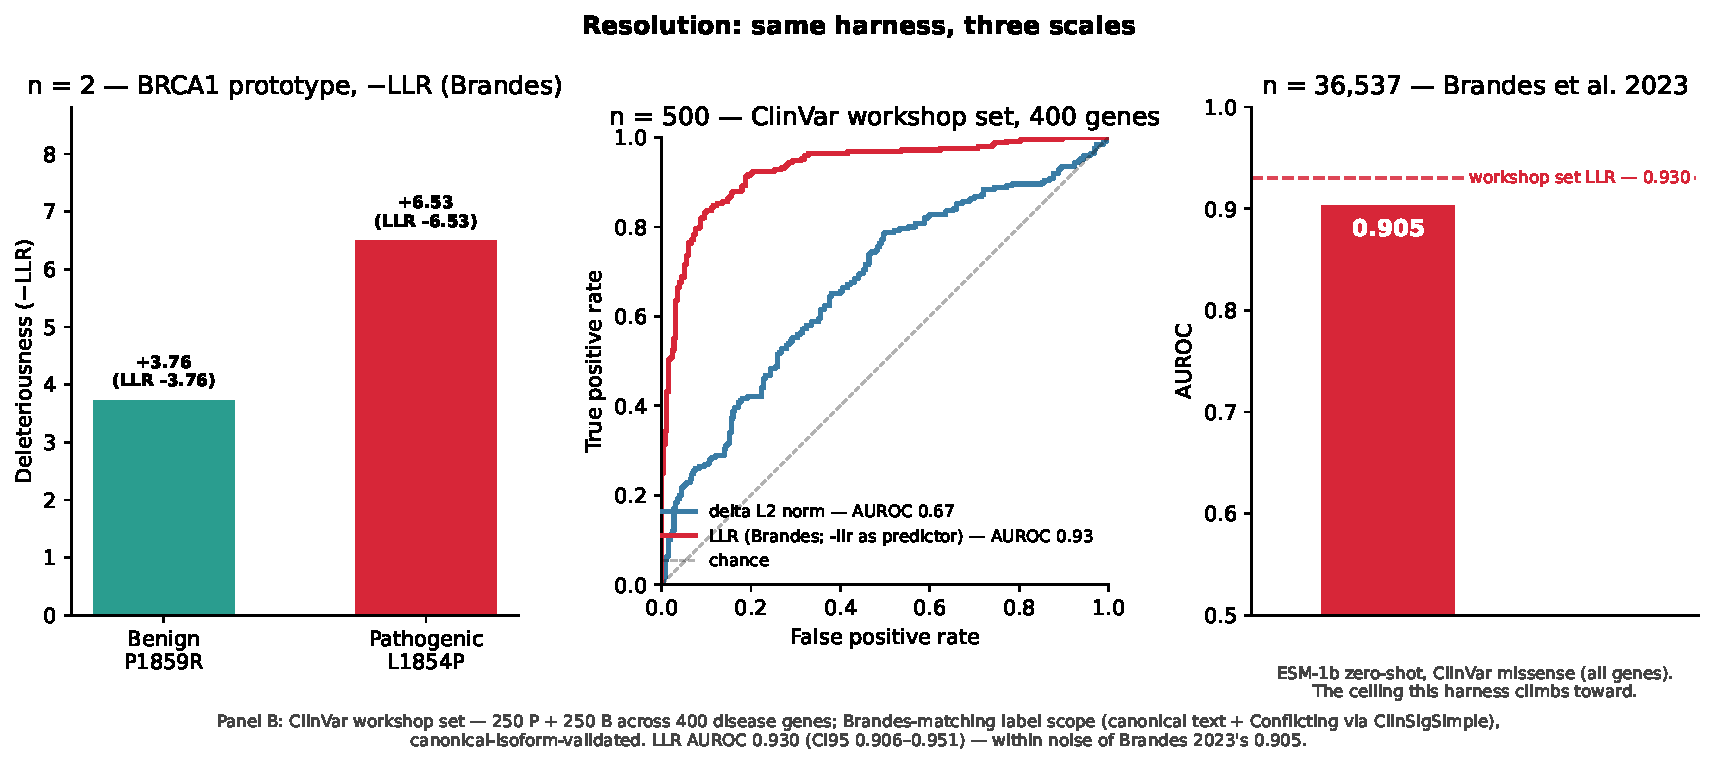
\includegraphics[width=\linewidth]{resolution_panels}
  \caption{% TODO(agent): caption per PROVENANCE.md :: §Results}
  \label{fig:resolution}
\end{figure}

\section{Discussion}
\label{sec:discussion}
% TODO(agent): see experiments/PROVENANCE.md :: §Discussion

\section*{Acknowledgments}

Thanks to Matt Scicluna, Aaron Wenteler, Joey Ton (Amii), Anjana Puliyanda
(Amii), the LRW contributors, and Amii. This paper, the experiments cited
within, and the harness used to produce both were authored in collaboration
with a Claude Code agent operating against the public
\texttt{lrw-vep-ub2026} repository.

\bibliographystyle{plainnat}
\bibliography{../shared/bib/references}

\end{document}
